\chapter{CMR\label{ch:cmr}}

In this chapter we present a concurrent memory reclamation scheme called \emph{CMR}.  We define the
problem of memory management carefully in \cref{sec:cmr-problem-def}, in order to get a complete
understanding of which problem we set out to solve.  In \cref{sec:cmr-overview} we present an
abstract overview of CMR, in order to get a high level understanding of the system as a whole,
without having to think about technical or implementation details.  \cref{sec:cmr-primitives}
discusses the primitives and operations of CMR, and how they are used.  Finally in
\cref{sec:cmr-correctness} we argue for the correctness of the system as presented in this chapter.
By reasoning about CMR without an implementation we later aim to show that the implementation
(\cref{ch:implementation}) fits the description of the system as we define it in this chapter.



\section{Problem Definition\label{sec:cmr-problem-def}}

We start by defining some central concepts. Memory $M$ is the set of all addresses in the address
space of the machine. A \emph{block} is a tuple $(a, n)$ and represents the memory segment
$\left[a, a + n\right)$. $M$ is a disjoint set $M = A \cap F$ where $A$ is the set of allocated
blocks, and $F$ is the remaining of the memory space. $F$ needs not, and is almost never, a
consecutive segments, but simply all memory that is outside any allocated block. We call such
memory \emph{invalid}, and all memory in an allocated block \emph{valid}.  We model the program
memory as a graph $G = (A, E)$ where $(u, v) \in E$ iff there is a pointer in $u$ pointing to an
address in the segment $v$. That is, memory blocks are the vertices, and pointers in the program
are the edges. See \cref{fig:memory-graph} for a possible memory layout with a graph.

\begin{figure}[ht]
  \centering
  \begin{subfigure}{0.45\textwidth}
    \begin{lstlisting}[style=Rust]
a = Node { value = 4, next = null }
b = Node { value = 8, next = a }
list = [a, b, 3]
    \end{lstlisting}
  \end{subfigure}
  \hfill
  \begin{subfigure}{0.45\textwidth}
    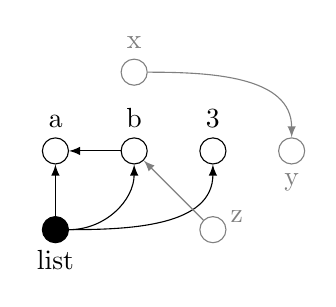
\begin{tikzpicture}[node distance=1cm]
  \node [draw,circle,label={a}]    (a)              {};

  \node [draw,circle,label={b}]    (b) [right of=a] {};
  \draw[-latex] (b.west) -- (a.east);

  \node [draw,circle,label={3}]    (3) [right of=b] {};

  \node [draw,circle,fill,label={[label distance=-0.8cm]:list}] (l) [below of=a] {};
  \draw[-latex] (l.north) -- (a.south);
  \draw[-latex] (l.east) to [out=0,in=270] (b.south);
  \draw[-latex] (l.east) to [out=0,in=270] (3.south);


  \node [draw,circle,color=gray,label={[color=gray]x}] (x) [above of=b] {};
  \node [draw,circle,color=gray,label={[color=gray,label distance=-0.8cm]y}] (y) [right of=3] {};
  \draw[-latex,color=gray] (x.east) to [out=0,in=90] (y.north);
  \node [draw,circle,color=gray,label={[right,xshift=1mm,color=gray]z}] (z) [below of=3] {};
  \draw[-latex,color=gray] (z) -- (b);
\end{tikzpicture}

  \end{subfigure}
  \caption{Code sample (left) with possible heap layout (right). If the black filled node is the
  only root, the black nodes are reachable, and the gray nodes are not.\label{fig:memory-graph}}
\end{figure}

As most programs need memory blocks of dynamic size, allocation and deallocation,
\emph{``freeing''}, is commonplace. The problem of memory management is to know when it is
\emph{safe} to free a memory block. We want to avoid the following memory hazards:

\begin{definition}[\egn{use-after-free\label{def:use-after-free}}]
  Memory that was allocated and then freed is read.
\end{definition}

\begin{definition}[\egn{invalid-read\label{def:invalid-read}}]
  Memory that has never been allocated is read.
\end{definition}

\begin{definition}[\egn{double-free\label{def:double-free}}]
  A block is freed twice without being allocated in between.
\end{definition}


\egn{use-after-free} is the most hazarous of the three, as program behaviour is often undefined
when freed values are read; in many language implementations undefined behavious means that the
entire program is illegal, and one cannot assume anything about its behaviour (see
\cref{sec:background-pl}). The consequence of \egn{use-after-free} usually ranges from reading
values that are unchanged from the time the block was freed, to mutation of memory that has been
reused.

\egn{invalid-access} is the least frequent of the three, as it requires the programmer to conjure a
pointer out of thin air, since it has never been allocated in the system. As with
\egn{use-after-free}, this is too is usually undefined, with similar consequences. Despite their
similarities we choose to have \egn{invalid-access} as a separate category, as pointer arithmetic
may lead to these hazards.

\egn{double-free} is technically not a memory hazard, as the operating system can check for the
validity of pointers that are freed, although this is often not done in practice. It is not clear
whether this is due to performance penalties of checking, or if it is primarily a legacy
bevhaviour; POSIXs definition of \code{free} states that it is undefined behaviour to pass a
non-allocated pointer to \code{free}\cite{posix}.

We aim to show that CMR guarantees that neither of the three memory hazards are possible.


\subsection{Shared Memory}

Newer languages like modern C++ and Rust aim to avoid having the programmer manage memory manually,
due to a long history of the consequences of memory hazards. For single threaded application, this
may be considered a problem with suggested solutions. Rusts ownership model and lifetime tracking
(\cref{ch:rust}), and similar methods from the C++ standard library, are proposed solutions.
However, the ownership model does not handle shared memory functionally, as objects in shared
memory might not have an owner responsible for its management. Despite not being a complete
solution, having ``solved'' single threaded memory management turns out to be of great help.

\begin{figure}[ht]
  \centering
  \begin{tikzpicture}
  \node [lnode,node distance=1.5cm] (n1)               {};
  \node [lnode,node distance=1.5cm] (n2) [right of=n1] {};
  \node [lnode,node distance=1.5cm] (n3) [right of=n2] {};
  \node [lnode,node distance=1.5cm] (n4) [right of=n3] {};

  \draw[ptr] ($(n1.east) - (0.25,0)$) -- (n2);
  \draw[ptr] ($(n2.east) - (0.25,0)$) -- (n3);
  \draw[ptr] ($(n3.east) - (0.25,0)$) -- (n4);
  \draw[ptr] ($(n4.east) - (0.25,0)$) -- ($(n4.east) + (0.4,0)$);

  \node [draw,fill=white,node distance=1.5cm, inner sep=0.2cm] (d1) [below of=n1,xshift=-0.19cm] {};
  \node [draw,fill=white,node distance=2cm,circle] (d2) [below of=n2,xshift=-0.19cm] {};
  \node [draw,fill=white,node distance=1.5cm] (d3) [below of=n3,xshift=-0.19cm] {$\pi$};
  \node [draw,fill=white,node distance=1.5cm] (d4) [below of=n4,xshift=-0.19cm] {\code{"hello"}};


  \draw[ptr] ($(n1) + (-0.19, +0.05)$) -- (d1.north);
  \draw[ptr] ($(n2) + (-0.19, +0.05)$) -- (d2.north);
  \draw[ptr] ($(n3) + (-0.19, +0.05)$) -- (d3.north);
  \draw[ptr] ($(n4) + (-0.19, +0.05)$) -- (d4.north);

  \node[draw,fill=white,circle,node distance=0.5cm] (treel) [below of=d2,left of=d2] {};
  \node[draw,fill=white,circle,node distance=0.5cm] (treer) [below of=d2,right of=d2] {};
  \draw[-latex] (d2) -- (treel);
  \draw[-latex] (d2) -- (treer);

  \node [draw,fill=white,node distance=2cm] (back) [left of=n1] {\code{0xcafe}};
  \draw[ptr] (back) ($(d1) + (0.05,0)$) to [out=180,in=270] (back.south);

  \begin{scope}[on background layer]
    \node [draw,fill=lightred!40, fit={(back) (n4)},inner sep=0.5cm] (shared-mem) {};
    \node [draw,fill=rust!60, fit={(d1) (treel) (d4)},inner sep=0.3cm] (shared-mem) {};
  \end{scope}

  \node (shared-label) [above of=back] {Shared memory};
  \node (rust-label) [below of=d4,xshift=-0.3cm] {Owned memory};
\end{tikzpicture}

  \caption{Example of memory layout showing owned memory (beige) and shared memory (red). Types in
  shared memory may contain pointers to owned memory, and vice versa.\label{fig:rust-shared-mem}}
\end{figure}

We divide up $A$ into two disjoint parts: \emph{owned} and \emph{shared} memory.  Owned memory is
all memory which management is already handled by some system, like Rusts ownership model or the
smart pointers of C++. Shared memory is the memory in which the structures that is not modeled well
by other constructs live, like the nodes in a linked list.

A key idea to recognize is that despite data being in Shared memory, they might themselves own data
that is in Owned memory, like the binary tree in \cref{fig:rust-shared-mem}. The destruction of a
list node containing the binary tree will utilize the system for owned memory, and make sure that
the binary tree is cleaned up properly. It does not matter if the list node itself resided in owned
or shared memory.  With this distiction we can reduce our problem space significantly, as we only
have to worry about the small subset of $A$ that is shared memory.  Note that it is also possible
to have the data types that are referenced from shared memory but stored in owned memory, like the
pointer poining to \code{0xcafe} in \cref{fig:rust-shared-mem}.  This includes pointers on a stack
frame, but might also include a entry in a hashmap. It is these pointers that CMR aims to control.


\section{Overview\label{sec:cmr-overview}}

We call a pointer from owned memory to shared memory for a \emph{root}.  CMR is based on the idea
that if we have access to all roots in the system at an instant, finding the set of all reachable
blocks $R$ from the set of roots $R_0$ is simple: $R$ is the transitive closure of ``there is a
pointer from $x$ to $y$'' on $R_0$.  We call identifying $R$ \emph{reachability analysis}. By
then tracking all allocated blocks $A$, we can identify the set of unreachable block $G$ by taking
the relative complement of $R$ in $A$: $G = A \setminus R$.

CMR tracks all roots for each thread by restricting where the roots may be stored in memory. This
way we know at any time where all roots in the process resides, so they can be collected by any
other thread with relatively low effort.


When performing the reachability analysis in a concurrent systems, simply following pointers while
maintaining a frontier of unvisited blocks is not sufficient. Since there are multiple threads in
the system, some other thread $T'$ may come along and change pointers, causing reachable blocks to
be observed as unreachable by the reclaiming thread, as shown in \cref{fig:pointer-swap}. After
having read the left child of some node with two children, the two pointers can be swapped by the
other thread, causing us to visit one of the nodes twice, as if the two child pointers point to the
same node. CMR handles this problem by obtaining a snapshot of the process memory, and performs
the reachability analysis on the snapshot.

\begin{figure}[ht]
  \centering
  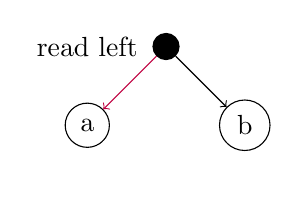
\begin{tikzpicture}
  \node [draw,fill,circle] (r) {};
  \node [draw,circle] (a) [left  of=r, below of=r] {a};
  \draw[->,color=purple] (r) -- (a);
  \node [draw,circle] (b) [right of=r, below of=r] {b};
  \draw[->] (r) -- (b);
  \draw[<->,color=white] (a) to [out=-45,in=-135] (b);

  \node () [left of=r] {read left};
\end{tikzpicture}
\hspace{1cm}
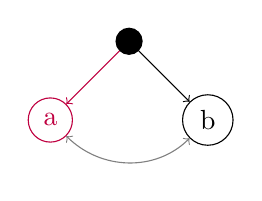
\begin{tikzpicture}
  \node [draw,fill,circle] (r) {};
  \node [draw,color=purple,circle] (a) [left  of=r, below of=r] {a};
  \draw[->,color=purple] (r) -- (a);
  \node [draw,circle] (b) [right of=r, below of=r] {b};
  \draw[->] (r) -- (b);
  \draw[<->,color=gray] (a) to [out=-45,in=-135] (b);
\end{tikzpicture}
\hspace{1cm}
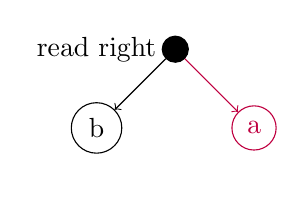
\begin{tikzpicture}
  \node [draw,fill,circle] (r) {};
  \node [draw,color=purple,circle] (a) [right  of=r, below of=r] {a};
  \draw[->,color=purple] (r) -- (a);
  \node [draw,circle] (b) [left of=r, below of=r] {b};
  \draw[->] (r) -- (b);
  \draw[<->,color=white] (b) to [out=-45,in=-135] (a);

  \node () [left of=r] {read right};
\end{tikzpicture}

  \caption{Mutation in the memory graph may lead to reachable blocks being observed as
  unreachable.\label{fig:pointer-swap}}
\end{figure}


The \proc{Reclaim} procedure shows how we reclaim memory in CMR\@. The input is the set of
allocated address $A$ and information on all threads $T$. In \proc{Get-Roots} we collect all roots
for all threads. \proc{Find-Reachable} runs the reachability analysis, and returns the set of all
reachable blocks $R$. We can then find $G$.

\begin{codebox}
\Procname{$\proc{Reclaim}(A, T)$}
\li $\proc{Snapshot}()$
\li $R_0 \gets \proc{Get-Roots}(T)$
\li $R \gets \proc{Find-Reachable}(R_0)$
\li $G \gets A \setminus R$
\li $\proc{Free}(G)$
\li $A \gets R$
\end{codebox}

\begin{codebox}
\Procname{$\proc{Find-Reachable}(R_0)$}
\li $\id{Frontier} \gets R_0$
\li $\id{Seen} \gets R_0$
\li \While $m \gets \proc{Pop}(\id{Frontier})$
\li   \Do \For $\id{ptr} \gets \proc{Pointers}(m)$
\li     \Do \If $\id{ptr} \notin \id{Seen}$
\li         \Do
            $\proc{Insert}(\id{Seen}, \id{ptr})$
\li	  		  $\proc{Push}(\id{Frontier}, \id{ptr})$
            \End
        \End
      \End
\li \Return $\id{Seen}$
\end{codebox}

\section{Primitives of CMR\label{sec:cmr-primitives}}

In this section we look at the four data types in CMR, and operations that act on them. All types
are generic over some type $T$, which is omitted for brevity. The operations on these types do not
change the generic type.

\begin{definition}[\egn{Guard}\label{def:guard}]
  \egn{Guard} is an object that either contains a root or \nullptr. The \egn{Guard} is non-movable
  in memory. All roots are stored in \egn{Guards}.
\end{definition}

\fixme{01/06 13:44 ``other systems''}
The \egn{Guard} is the only type that CMR defines that are different from other systems, and we
only use \egn{Guard}s to limit the storage of roots.

\begin{definition}[\egn{Atomic}\label{def:atomic}]
  \egn{Atomic} is a pointer type that provides safe concurrent access to its users.
\end{definition}

\egn{Atomic} is similar to regular atomic pointers from any programming language; it offers safe
reads and writes for concurrent systems.

\begin{definition}[\egn{NullablePtr}\label{def:nullable-ptr}]
  \emph{NullablePtr} is an immutable pointer that may be \nullptr. It is obtained through a Guard.
  When a NullablePtr $p$ is obtained from a Guard $g$, $g$ is immutable thoughout the
  lifetime\footnote{We use the same meaning of lifetime as Rust (\cref{sec:rust-lifetimes})}
  of $p$.
\end{definition}

The definition of \egn{NullablePtr} is important: it shows that we scope the immutability of a
\egn{Guard} to the lifetime of the \egn{NullablePtr}; this allows us to have certain invariants
that hold in between changes to a \egn{Guard} to hold for the lifetime of an \egn{NullablePtr}.

\begin{definition}[\egn{Ptr}\label{def:ptr}]
  \egn{Ptr} is an immutable pointer that may not be \nullptr. All accesses to shared memory is
  through a Ptr.
\end{definition}
The semantics of \egn{Ptr} are similar to that of \egn{NullablePtr}, but the two are distinct types
for simplification of the \nullptr-case.


\subsection{Operations}

A Guard can be constructed with the initial value of $\bot$ with \emph{make-guard}
\begin{equation}\label{eq:make-guard}
  \proc{Make-Guard}\typeof{} () \to \id{Guard}
\end{equation}
It can also copy the value of another Guard with \emph{copy-guard}.
\begin{equation}\label{eq:copy-guard}
  \proc{Copy-Guard}\typeof{} (\id{Guard}, \id{Guard}) \to ()
\end{equation}

General usage of \egn{Guard} is to construct the number of \egn{Guard}s one needs for some operation.
These \egn{Guard}s are then used to load \egn{Atomic}s into.

Atomic is a regular atomic pointer variable, supporing operations such as \emph{store}, and
\emph{compare-and-swap}.
\begin{equation}\label{eq:atomic-store}
  \proc{Store}\typeof{} (\id{Atomic}, \id{NullablePtr}) \to ()
\end{equation}
\begin{equation}\label{eq:atomic-cas}
  \proc{Compare-And-Swap}\typeof (\id{Atomic}, \id{NullablePtr}, \id{NullablePtr}) \to
  \id{NullablePtr}
\end{equation}

It is not safe to \emph{load} an atomic, as there is no guarantee that the
pointer read is protected by a guard. Instead, CMR defines \emph{load-atomic}, which loads an
Atomic into a Guard, and returns the value read as a NullablePtr:
\begin{equation}\label{eq:load-atomic}
  \proc{Load-Atomic}\typeof{} (\id{Guard}, \id{Atomic}) \to \id{NullablePtr}
\end{equation}

The NullablePtr is just a convenience type in order to not have to handle the $\bot$ case of all
pointers. Whether the pointer is null or not can be checked:

\begin{equation}\label{eq:nullable-is-null}
  \proc{Is-Null}\typeof (\id{NullablePtr}) \to \id{bool}
\end{equation}

Ptr may be used in the place of NullablePtr, since is it just a special case of it. All functions
that take a NullablePtr can also take a Ptr.



\subsection{Pointer Tagging}

CMR also supports using the lower bits of a pointer to store extra information (a \emph{tag}). This
is useful for implementing deletion in linked lists, among other things. The tag is read with
\emph{tag},
\begin{equation}\label{eq:ptr-tag}
  \proc{Tag}\typeof{} (\id{NullablePtr}) \to \id{int}
\end{equation}
and a new NullablePtr can be constructed with a given tag using \emph{with-tag}.
\begin{equation}\label{eq:ptr-with-tag}
  \proc{With-Tag}\typeof{} (\id{NullablePtr}, \id{int}) \to \id{NullablePtr}
\end{equation}
The actual address of the pointer is obtained through \emph{addr}
\begin{equation}\label{eq:ptr-addr}
  \proc{Addr}\typeof{} (\id{NullablePtr}) \to \id{int}
\end{equation}



\section{Correctness\label{sec:cmr-correctness}}

Having defined the types and operations that CMR provides we prove important properties of the
system.

\begin{theorem}[\egn{Guard} is valid]\label{thm:guard-valid}
  If a \egn{Guard} is not $\bot$, it points to valid memory.
\end{theorem}
\begin{proof}
  \todo{this}
\end{proof}

\begin{lemma}[\egn{Ptr} is valid]\label{lm:ptr-valid}
  The \egn{Ptr} points to valid memory.
\end{lemma}
\begin{proof}
  The  \egn{Ptr} $p$ is read from a \egn{Guard} $g$ and $g$ is immutable throughout the lifetime of
  $p$ so they have the same value. $p \neq \bot$, so this follows by \cref{thm:guard-valid}.
\end{proof}

\cref{lm:ptr-valid} is the most important result in this section, since it guarantees that
accesses of the memory in a \egn{Ptr} is valid. Thus, a memory access through a \egn{Ptr} can not
result in a invalid-read (\cref{def:invalid-read}) or use-after-free (\cref{def:use-after-free})
hazard.

\begin{lemma}
  CMR has no \egn{use-after-free} or \egn{invalid-read}
\end{lemma}
\begin{proof}
  This follows from \cref{lm:ptr-valid} as all accesses to shared memory are through a \egn{Ptr}
  (\cref{def:ptr}).
\end{proof}

\begin{lemma}
  CMR has no \egn{double-free}
\end{lemma}
\begin{proof}
  $G \gets A \setminus R$ so only allocated addresses are freed. $A_{i+1} \gets R$, so freed
  addresses are discarded from $A$ in each call to \proc{Reclaim}.
\end{proof}
